\documentclass[a4paper,10pt]{article}
\usepackage[utf8]{inputenc}
\usepackage{url}
\usepackage{amsthm, amscd, amsfonts, amssymb, graphicx,tikz, color, environ}

%opening
\title{Literature Review: Simulating Flexible Assembly System Event Logs for the Purposes of Process Modelling and Machine Learning – DRAFT}
\author{Tero Keski-Valkama}

\begin{document}

\maketitle

\smallskip
\noindent \textbf{Keywords.} Flexible Assembly System, Simulation

\section{Topic}
Flexible Assembly System is a modular and reconfigurable assembly and tooling workshop with a focus on small and medium-sized batches of varying products.
Flexible Assembly System was described formally by Donath and Graves \cite{donath1988flexible} as a system consisting of a set of products each with a specified volume
assembled on a workshop consisting of a fixed number of cells.

The assembly steps are performed in cells in parallel. Assemblies and components are transported to the cell where they are combined, tooled or inspected. Products
are transported out of the cell for the next assembly step in another cell, or out of the system as end products.
The work steps executed in the cells can be manual or automatic. There can be a central storage such as a shelf for storing components, the intermediate assemblies between the steps
and the end products waiting to be transported out of the system.

Flexible Assembly System work loads consist of small and medium sized batches where there can be some variation in the products based on customization and personalization.
The Flexible Assembly Systems are modular and often composed out of independent modules from different suppliers. The Flexible Assembly System event trace consists
of events received from all the separate modules of the system, and additional sensors and triggers added to the system in integration phase or later.

Using a Flexible Assembly System to assemble batches of products generates an electronic event trace which is logged. The events in the event trace are typically at least
partially agnostic to the assembly process being performed, and therefore the events do not include tokens connecting the event to a specific final product instance.

Simulating these kinds of event traces provides valuable material for learning systems which can be used to derive assembly process models and to detect deviances.

\section{Description of Method}

A proper literature review is a methodological, continuous process. The goal of the literature review is to accumulate a body of relevant existing knowledge
about the topic, categorized based on subtopics and keywords.
Ultimately the literature review can be presented in the article in a summary form to present the context of the research.
The collected references represent a focused area of the existing literature relevant to the object of research.

The review starts from discovery, discovering information sources and starting points of review. The literature review process progresses towards synthesis
where the relevant existing knowledge is synthesized together to form an understanding of the composite.

The discovery phase includes a listing of subtopics and keywords, to structure the gathered discovered information into a manageable form. The goal
of the discovery phase is to form questions about the existing knowledge and to find answers to them.

The synthesis is composed of the description of the existing knowledge and possible gaps related to the research.

\section{Discovery Phase}

The topic under review is somewhat cross-discplinary relating to industrial assembly processes, business process modelling and learning systems.
Overall the following subtopics are recognized:
\begin{enumerate}
 \item Assembly process modelling and simulation
   \begin{enumerate}
     \item Fault modelling and simulation
   \end{enumerate}
 \item Mathematical analysis of log data
   \begin{enumerate}
     \item Analysing interleaved event traces
     \item Analysing delays and intervals
   \end{enumerate}
 \item Process mining
 \item Visualization of event logs
\end{enumerate}

\begin{figure}[h]
\begin{center}
 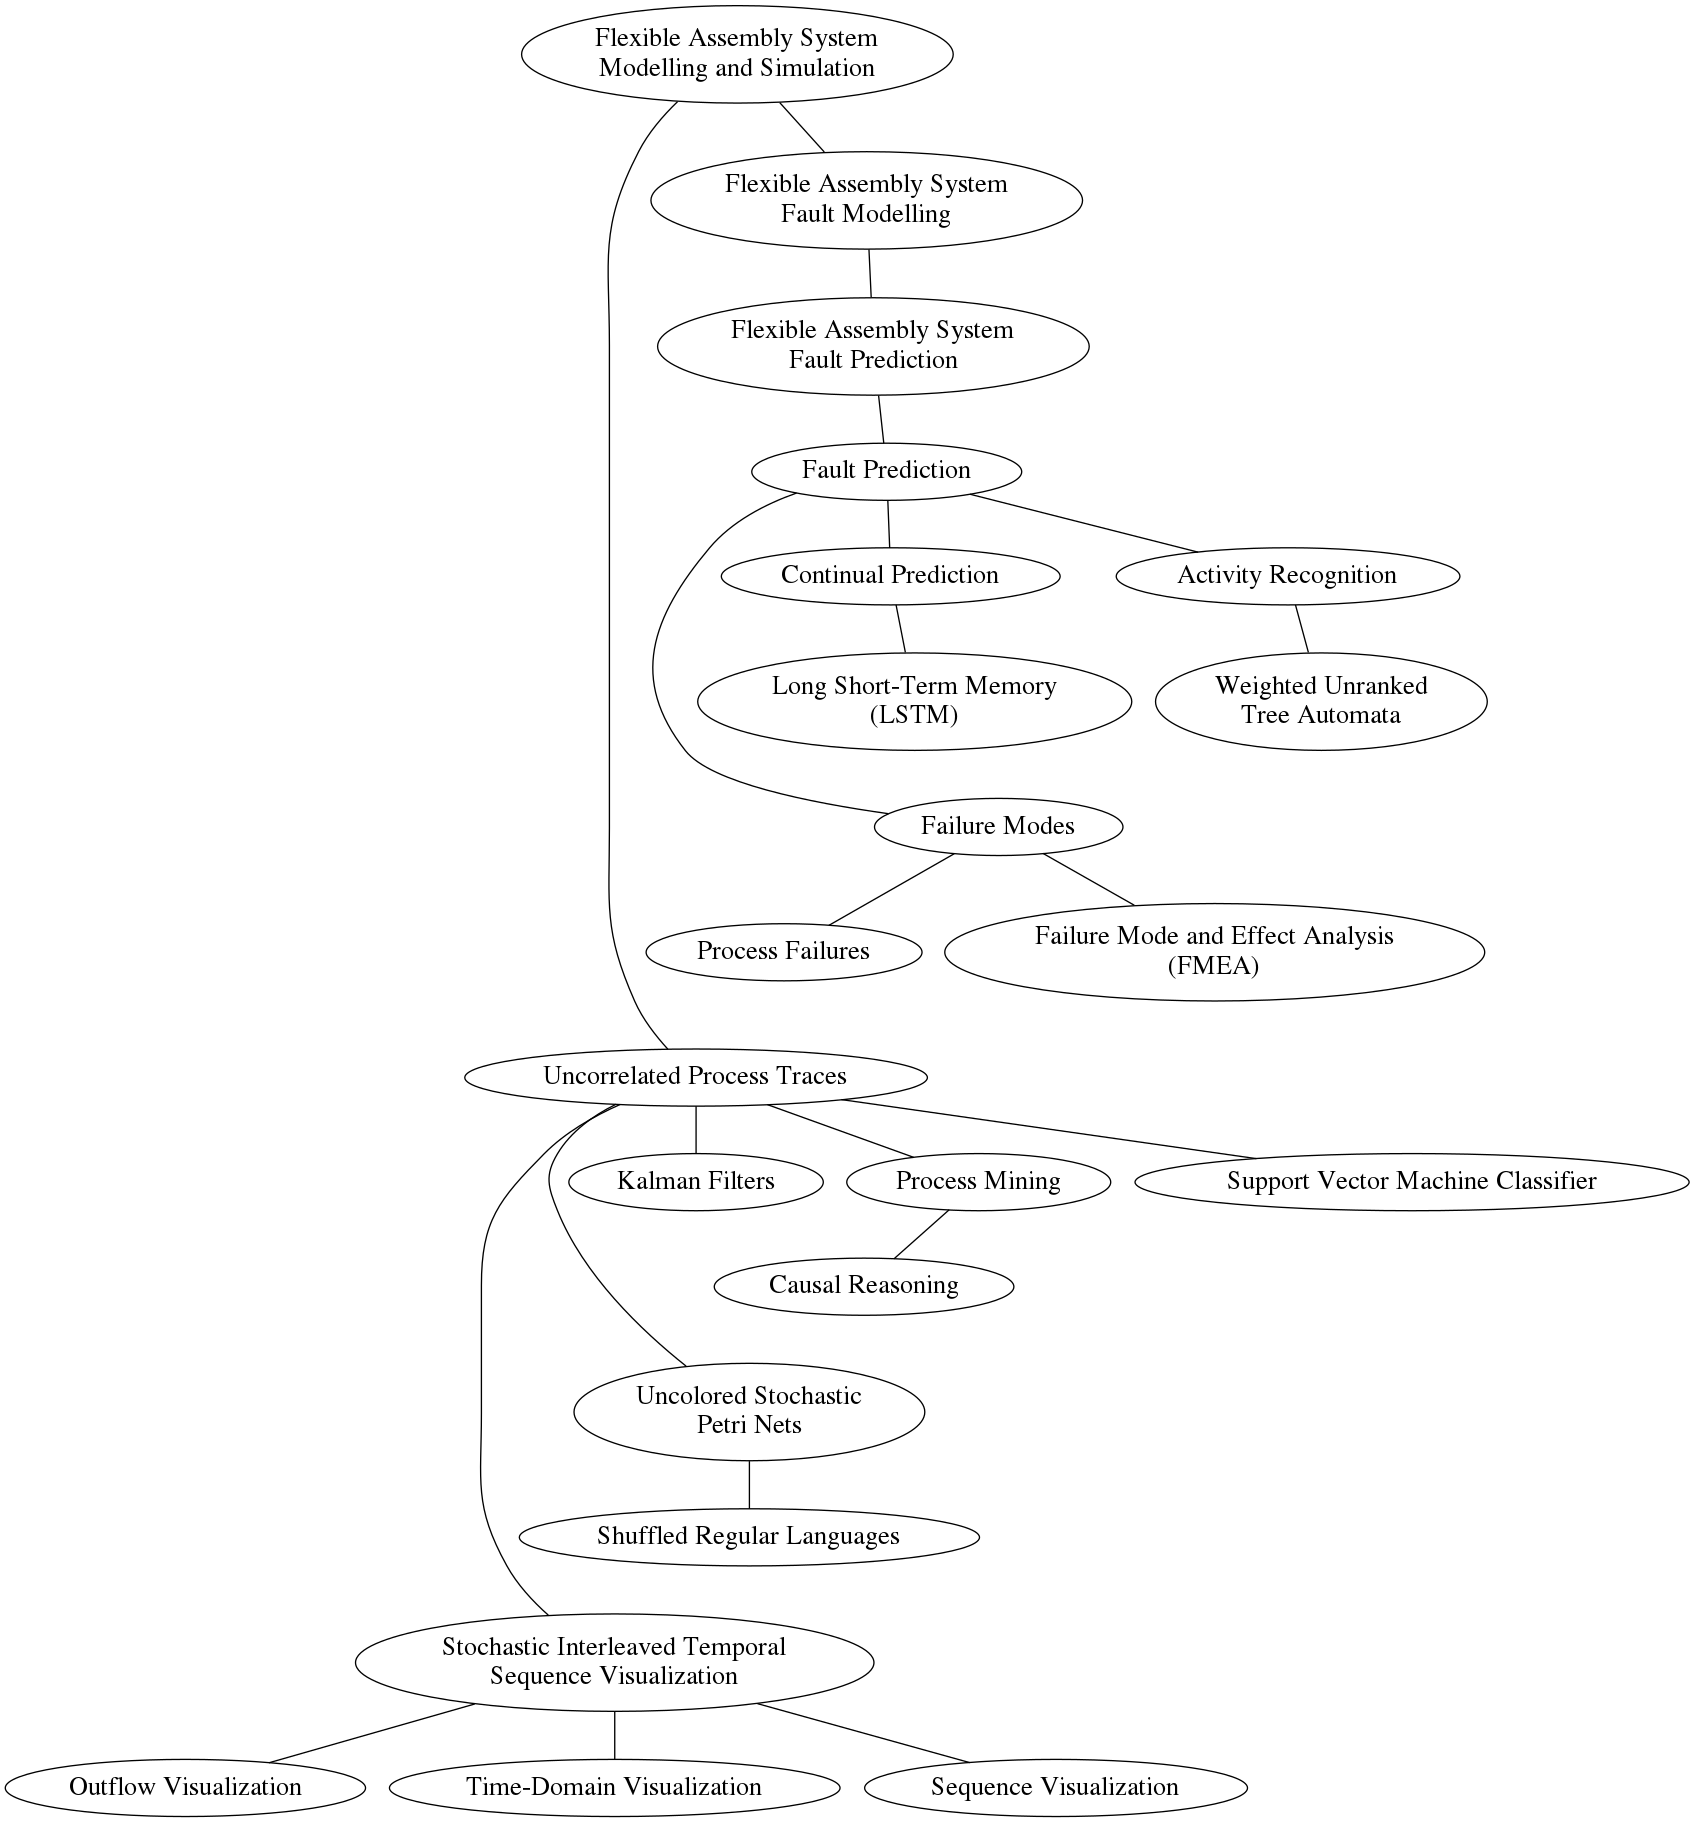
\includegraphics[width=\textwidth]{./field.png}
 % field.png: 0x0 pixel, 300dpi, 0.00x0.00 cm, bb=
\end{center}
\caption{The mind map of the research topic}
\end{figure} 

\subsection{Keywords}

The keywords relevant for the research were collected from a set of articles deemed especially relevant for this research. A representative set of articles was
read and relevant keywords were picked from titles, abstracts and references. This set of keywords allows for directed browsing of relevant literature.

\begin{itemize}
 \item assembly process
 \item assembly system
 \item complex robotic system
 \item compliant parts
 \item dimensional quality
 \item dimensional variation propagation
 \item discrete event system
 \item Failure mode and effects analysis (FMEA)
 \item failure rates
 \item failure records
 \item failure report
 \item fault detection
 \item fault mode
 \item fixture variation
 \item interleaving
 \item leaf spring
 \item multiple failure modes
 \item Multi-Station Assembly Systems
 \item outflow visualization
 \item part variation
 \item petri nets
 \item process control
 \item process failures
 \item process FMEA
 \item reduction of irregularities
 \item reliability
 \item simulation
 \item time-domain visualization
 \item uncolored petri nets
 \item variation propagation
 \item visualization of sequences
 \item welding gun variation
\end{itemize}

The core questions about the existing literature are:
\begin{enumerate}
 \item What methods are there to model and simulate assembly processes and related faults?
 \item What methods are there to visualize event logs with or without timestamps?
 \item What are the relevant keywords and terms to describe this problem space?
\end{enumerate}

\section{Synthesis}

Assembly systems, construction processes and business processes are often simulated using discrete event simulation, for example in:
\cite{hlupic1998business,zhao2010efficient,kang2013active,rahnama2010fuzzy}. These simulations are used for process optimization\cite{sadeghi2008framework}, scheduling and
assembly line design. The models of these systems are conveniently described using Process algebra Petri nets (PPNs) \cite{falkman2007specification}.

The literature about faults and deviances in assembly processes mainly focus on the faults in the assembled products.
There are less academic publications about simulating process deviances in assembly processes such as unexpected process failures, human errors, and deadlocks.

The model of the simulated system is created in production line design \cite{bullinger}, by observing the system, or by interviewing the system specialists \cite{montevechi2012using}.

A discrete event simulation output is a sequence of generated events,
and the internal system state between the events. The sequence of generated events is useful as a corpus for learning algorithms if it reflects the real conditions and
target phenomena well enough. In the case of fault detection, the simulation should be representative for the correct operation of the target system, and deviances
are in principle.

Process mining is the field of inferring the underlying business processes based on observed events and transitions. The process mining methods can be used
to compare the supposed process model with the observed processes to detect deviances.
Parallel processes create interleaved process traces.
The methods for describing process traces in the context of process mining are loosely based on the alpha algorithm and as such, they all expect process instances
to be identified in the activity events to deinterleave the process traces and to infer causal relations of activities.

\bibliographystyle{IEEEtran}
\bibliography{LiteratureReview}

\end{document}
